\documentclass[tikz]{standalone}
\begin{document}
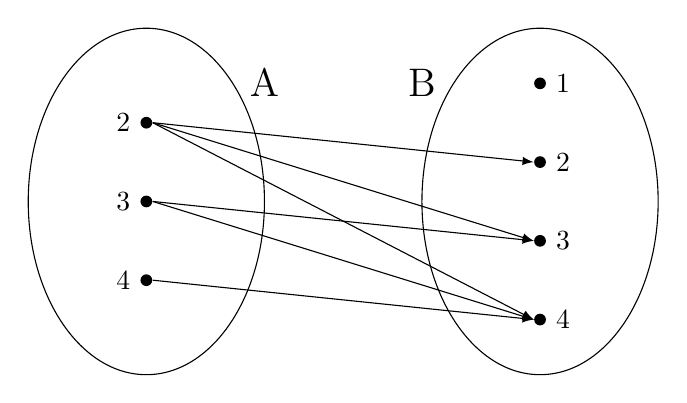
\begin{tikzpicture}[>=latex]
    
    % --- Set A on the left ---
    \draw (0, 1.0) ellipse (1.5cm and 2.2cm);

    % Label 'A' above and to the left of the set
    \node at (1.5, 2.5) {\Large A};

    % Points in set A, stacked vertically
    \node[circle, fill, inner sep=1.5pt, label=left:2] (a2) at (0, 2.0) {};
    \node[circle, fill, inner sep=1.5pt, label=left:3] (a3) at (0, 1.0) {};
    \node[circle, fill, inner sep=1.5pt, label=left:4] (a4) at (0, 0.0) {};

    % --- Set B on the right ---
    \draw (5, 1.0) ellipse (1.5cm and 2.2cm);

    % Label 'B' above and to the left of the set
    \node at (3.5, 2.5) {\Large B};

    % Points in Set B, stacked vertically and alligned to match poitns in A where possible
    \node[circle, fill, inner sep=1.5pt, label=right:1] (b1) at (5, 2.5) {};
    \node[circle, fill, inner sep=1.5pt, label=right:2] (b2) at (5, 1.5) {};
    \node[circle, fill, inner sep=1.5pt, label=right:3] (b3) at (5, 0.5) {};
    \node[circle, fill, inner sep=1.5pt, label=right:4] (b4) at (5, -0.5) {};

    % --- Arrows representing the connections (relation) ---
    % The arrows go from the east side of points in A to the west side of points in B
    
    % Connections from point 2 in A
    \draw[->] (a2.east) -- (b2.west);
    \draw[->] (a2.east) -- (b3.west);
    \draw[->] (a2.east) -- (b4.west);
    
    % Connections from point 3 in A
    \draw[->] (a3.east) -- (b3.west);
    \draw[->] (a3.east) -- (b4.west);
    
    % Connection from point 4 in A
    \draw[->] (a4.east) -- (b4.west);
\end{tikzpicture}
\end{document}